\mysubsection{Задача оптимальной торговли зерном}

В качестве базовой модели выбрана задача, предложенная в книге Suresh P. Sethi, Gerald L. Thompson.  Optimal control theory: applications to management science and economics, раздел 6.2.\cite{b8}

Цель данной задачи состоит в максимизации общей стоимости активов трейдора, к конечному моменту временного интервала.

Рассмотрена фирма, основной вид деятельности трейдинг (покупка, продажа) зерна на бирже. Активы фирмы составляют – денежные средства и материальные активы (пшеница). Волатильность зерновых цен на бирже, может оказывать непосредственное влияние на балансовые активы фирмы. 

Цель фирмы - максимизация общей стоимости активов на заданном горизонте времени $T$, путем покупки и продажи пшеницы.


Если фирма хранит слишком много активов в денежном эквиваленте, то она теряет деньги с точки зрения альтернативных издержек, поскольку она может получить более высокую прибыль, покупая  зерно на бирже.

С другой стороны, если остаток денежных средств слишком мал, фирма должна продавать материальные активы, чтобы удовлетворить спрос на денежные средства.

Задача состоит в том, чтобы найти оптимальное поведение фирмы (трейдера) на бирже.

Для постановки задачи оптимального управления введем следующие обозначения:\\
\begin{math} T \end{math} --- горизонт времени,\\
\emph {х}(\emph{t}) --- остаток денежных средств в момент времени $t$ (фазовая переменная),\\
\emph {у}(\emph{t})  --- баланс пшеницы в бушелях в момент времени $t$ ( 1 бушель пшеницы = 27,216 кг)(фазовая переменная),\\ 
${v(t)}$ --- скорость покупки пшеницы в бушелях за единицу времени, может быть положительной и отрицательной; отрицательная покупка означает продажу (управление),\\
\emph {р}(\emph{t}) --- цена пшеницы за бушель в момент времени $t$,\\
${r}$ --- постоянная положительная процентная ставка, на остаток денежных средств на счете,\\
\emph {h}(\emph{y}) --- функция затрат на хранение пшеницы.
 
Фазовые переменные $x$ и $y$ могут принимать отрицательные значения, таким образом, допускаются заимствование денег и короткие продажи пшеницы.



Запишем динамическую систему:
\begin{align}
    \Dot{x} & = r x(t) - h(y) - p(t) v(t),\, x(0) = x_{0}, \label{f1} \\
    \Dot{y} & = v(t), \, y(0) = y_{0} \label{f2}\\
    - v_2 & \le v(t) \le v_1, \label{f3}
\end{align}    
где $v_{1}$ и ${v_2}$ неотрицательные постоянные. 

Задача состоит в том, чтобы максимизировать целевой функционал

\begin{align}
    J = x(T) + p(T) y(T)\to \mathrm{max}
\end{align} 
при ограничениях (\ref{f1}) - (\ref{f3}). Обратим внимание, что задача записана в форме Майера. В случае линейности функции  \emph{h} будем иметь линейную задачу оптимального управления, в которой Принцип максимума Понтрягина дает необходимое и достаточное условие оптимальности.

\mysubsection{Анализ с помощью  Принципа максимума Понтрягина}

Составим функции Понтрягина и концевую функцию Лангранжа: 
\begin{align}
    {H} & = \psi_{1} (r x - h(y) - p v) + \psi_{2} v,\\
    \mathcal{L} & = \alpha_{0} (-x(T) - p(T) y(T)).
\end{align} 


Запишем сопряженную систему и условия трансверсальности:

\begin{gather}
 \Dot{\psi_{1}} = -H_x = -r \psi_{1},\label{f7}\\
\Dot{\psi_{2}} = -H_y = h'(y) \psi_{1},\label{f8}\\ 
    {\psi_{1}(T)} = - {L}_x(T)=\alpha_{0},\label{f9}\\
    {\psi_{2}(T)} = - {L}_y(T)=\alpha_{0} p(T) \label{f10}.
\end{gather} 

Легко видеть, что $\alpha_{0} > 0 $. Предположим, что $ \alpha_{0} = 0$ откуда следует\\ $\psi_{1} \equiv 0, \psi_{2} \equiv 0 $ тогда получаем противоречие. Таким образом, условия (\ref{f9}), (\ref{f10})  примут вид $\psi_1(T) =1,$  $\psi_2(T)=p(T)$.

Условие максимума функции Понтрягина для выбора управления ${v}$: 
\begin{gather}
    (\psi_{2} - \psi_{1} p)v\to \mathrm{max} \label{f11}.
\end{gather} 

Функция переключения:
\begin{align}
g = g(\psi_1 , \psi_2, p)=(\psi_{2} - p \psi_{1}).
\end{align} 


<<Bang-bang>>    функция определяется следующим образом:


\begin{align} \label{f13}
v^*(\psi_1 , \psi_2, p) = 
 \begin{cases}
   v_{1}, & \textrm{ при $g>0$.}\\
   -v_{2}, &  \textrm{ при $g<0$,}\\
   [-v_{2},v_{1}], & \textrm{ при $g=0$}.
 \end{cases}
\end{align}

Дадим следующую экономическую интерпретацию двойственным переменным и соотношениям принципа максимума:\\
 сопряженная переменная $ \psi_1(t) $ --- это теневая цена в момент времени ${t}$ одной денежной единицы, хранящейся на денежном счете,\\
 сопряженная переменная $ \psi_2(t) $ --- это теневая цена одного бушеля в момент времени ${t}$.
 
 
Уравнение (\ref{f7}) показывает, что при положительной ставке $ r>0 $ теневая цена денежных средств падает по экспоненте с коэффициентом $r$ в степени, т.е.  денежные средства обесцениваются с течением времени ввиду сокращения временного периода получения потенциального пассивного дохода.


Из уравнения (\ref{f8}) вытекает, что теневая цена пшеницы растет пропорционально предельным издержкам на хранение пшеницы (с учетом теневой цены денежных средств).


Из условия максимума (\ref{f11}) \big( cм. также (\ref{f13})\big) вытекает, что  ${v^*}$ --- это скорость продажи, покупки или бездействия трейдера на бирже при условии оптимальной стратегии, продавать по максимально доступной  ставке стоимости бушеля, или покупать, если стоимость бушеля складывается выгоднее стоимости денежных средств.


В случае если теневая цена бушеля с учетом стоимости хранения точно равна биржевой стоимости бушеля, оптимальная стратегия трейдера на бирже не определяется из Принципа максимума.


Исследуем этот вопрос более подробно.

\textbf{Анализ на наличие особых (магистральных) режимов на оптимальном процессе.}

Особые режимы характеризуются тем, что функция переключения $g \equiv 0$ на некотором интервале $[\tau_1, \tau_2]$ :
\begin{gather*}
  \psi_2 (t) = p(t) \psi_1 (t),\\
   \Dot{g} = 0 \Rightarrow  \Dot{\psi_2}(t) - \Dot{p}(t) \psi_1 (t) - p(t) \Dot{\psi_1}(t) = 0 \Rightarrow 
   \end{gather*}
   \begin{gather*}
  \Rightarrow h'(y(t)) \psi_1 (t) -   \Dot{p}(t) \psi_1 (t) + r p(t) {\psi_1}(t) = 0 \Rightarrow \\
  \Rightarrow  \psi_1 (t) \big[  h'(y(t)) -   \Dot{p}(t) + r p(t) \big] = 0 
\end{gather*}



Из уравнения (\ref{f7}) и условия трансверсальности $\psi_1(T)= 1$ следует, что $\psi_1(t)>0$  $ \forall t  \Rightarrow$ особый режим возможен лишь в случае, когда совместима система:\\
\begin{align}
 \begin{cases}
\psi_2(t) = p(t)\psi_1(t),  \\
h'(y(t)) - \Dot{p}(t)+r p(t) = 0
\end{cases}
\end{align}\\

Рассмотрим частный (но важный для дальнейшего изложения) случай:  $ {h(y)} = \frac{1}{2}|y|$, $ {r} = 0, $ функция \emph {р}(\emph{t}) кусочно-постоянная, при этом вместо производной, $h$ будем использовать элементы (субградиенты) субдифференциала Кларка:

\begin{align} \label{f15}
\partial h(y) =
 \begin{cases}
 \big\{\frac{1}{2}\big\}, & y>0,  \\
 \big\{-\frac{1}{2}\big\},& y<0, \\
\big[-\frac{1}{2}, \frac{1}{2} \big],& y=0.
\end{cases}
\end{align}\\



Очевидно, что на участках постоянства функции \emph {р}(\emph{t}) система (\ref{f15}) выполняется лишь при условии $ y(t) \equiv 0$, чему соответствует управление $ v(t) \equiv 0$.\\
Таким образом, в указанном частном случае задачи, оптимальное управление может принимать только 3 значения: $ \{ - v_2, v_1, 0\}$. Причем "внутреннее" значение $v(t) = 0$ возможно лишь тогда, когда выполняется условие:
\begin{displaymath}
\left\{ \begin{array}{ll}
 \psi_2(t) = p(t),\\
 y(t) \equiv 0.
  \end{array} \right.
\end{displaymath}

Заметим, что такой же вывод имеет место в случае квадратичной функции $ h(y) = c y^2 $ $(c>0)$.
 
 
\mysubsection{Модель продолжительной торговли пшеницей}
Уравнения (\ref{f1}), (\ref{f2}) и (\ref{f13}) определяют двухточечную краевую задачу, которая обычно требует процедуры численного решения. В этом разделе предполагается специальная форма для функции хранения ${h (y)}$, чтобы иметь возможность получить решение в замкнутой форме.

В данном случае мы используем следующие условия:\\
функция затрат на хранение пшеницы $$ {h(y)} = \frac{1}{2}|y|$$
нулевая процентная ставка $$ {r} = 0, $$
наличие денежных средств в начальный  момент времени $t=0$ $$ {x(0)} = 10, $$
баланс пшеницы в бушелях в момент времени $t = 0$ $$ {y(0)} = 0, $$
скорость покупки пшеницы в бушелях за единицу времени, может быть положительной и отрицательной; отрицательная покупка означает продажу: $$ {v_{1}} = {v_{2}} = 1, $$
горизонт времени $$ {T} = 6, $$
цена пшеницы за бушель в момент времени $t$:

\begin{displaymath}
p(t) =\left\{ \begin{array}{ll}
 3, & \textrm{если $0 \le t\le 3,$}\\
 4, & \textrm{если $4  \le t  \le 6.$}
  \end{array} \right.
\end{displaymath}\\


Будем применять Принцип максимума Понтрягина:\\

Запишем динамическую систему:
\begin{align}
    \Dot{x} & = - \frac{1}{2}|y| - p(t) v(t),\,\; x(0) = 10, \\
    \Dot{y} & = v(t), \,\; y(0) = y_{0},\\
    - v_2 & \le v(t) \le v_1.
\end{align}     

Составим понтрягиан: 
\begin{align}
{H} & = \psi_{1} (- \frac{1}{2}|y| - p(t) v(t)) + \psi_{2} v
\end{align} 

Запишем условия на сопряженные переменные:
\begin{gather}
 \Dot{\psi_{1}} = -H_x = 0,\\
 \Dot{\psi_{2}} = -H_y =  \frac{1}{2}\frac{|y|}{y}, \label{f21}\\
    {\psi_{1}(6)} = 1,\\
    {\psi_{2}(6)} = 4.\label{f23}
\end{gather}
Условия максимума функции Понтрягина:

\begin{align}
    (\psi_{2} - \psi_{1} p)v\to \mathrm{max}.
\end{align} 

Анализ покупки и продажи зерна на предложенном горизонте времени:


Функция переключения:

\begin{align}
g= g(\psi_1 , \psi_2, p) = (\psi_{2} - \psi_{1} {p}).
\end{align} 

<<Bang-bang>> функция определяется следующим образом:

\begin{align} \label{f26}
v^*(\psi_1 , \psi_2, p) = 
 \begin{cases}
   1, &\textrm{ при $g>0$},\\
   -1, &\textrm{при $ g<0$},\\
   [-1,1], &\textrm{при $g=0$}.
 \end{cases}
\end{align}

Таким образом, ${v^*} = 1$   скорость покупки бушеля, ${v^*} = -1$  скорость продажи бушеля, ${v^*  \in (-1, 1)} $ бездействие трейдера на бирже зерна.\\
 
На промежутке времени [0, 6] определим временной период: $ \Delta_{1} = [0,3)$, на котором: 
\begin{gather*}
\psi_{2}(t) = p(t),\\
\Dot{g} = 0 \Rightarrow \Dot{\psi_{2}}(t) = \Dot{p}(t) = 0, \\
\psi_{2} = 3,\;\, y = 0,\;\,  v = 0. 
\end{gather*}
Далее определим временной период: $ \Delta_{2} = [3,4]$:
\begin{gather*}
\psi_{2}(t) = p(t),\\
\Dot{g} = 0, \;\, \psi_{2} = 4, \\
y = 0, \;\,
v = 0.
\end{gather*}
При $ на t \in [0,1] \Rightarrow \psi_2(t) = p(t) = 3  $ от сюда следует, что c момента  $t^*$ начинаются покупки.
\begin{gather*}
{v} = 0, \;\, {y} = 0,\;\, \Dot{\psi_2} > 0  \Rightarrow\\
\Rightarrow g>0 \Rightarrow v^* = 1 , \;\, v = 1 \Rightarrow \\
\Rightarrow y(t) = t - t^*,\,\; t^*>1
\end{gather*}


\begin{gather*}
\psi_2(t) =
 \begin{cases}
3, &\textrm {если $ t \in [0, t^*], $}  \\
\frac{1}{2}t + 3 - \frac{1}{2}t^*, &\textrm {если $ t>t^*, $}
\end{cases}
\end{gather*}

введем момент времени $t^{**}$ конца продаж. Тогда
\begin{gather*}
\psi_2 (t^{**}) = \frac{1}{2}t + 3 - \frac{1}{2}t^* = 4,
\end{gather*}

\begin{gather}
t^{**} - t^* = 2, \label{f27 }\\
t^*>1 \Rightarrow t^{**}> 3,\nonumber
\end{gather}

\begin{gather*}
y(t) =
 \begin{cases}
 0, & \textrm{если $t \in [0, t^*],$ }\\
 t - t^*, & \textrm{если $ t > t^*. $}
  \end{cases}\\
\end{gather*}


Предположим, мы начинаем покупать пшеницу при $t^*> 1$. Из (\ref{f26}) коэффициент покупки равен 1; очевидно, что покупка будет продолжаться с такой скоростью.
При достижение  $t= 3$ покупка бушеля зерна прекращается.
Учитывая затраты на хранения зерна, для минимизации финансовых потерь, зерно должно быть продано в течение 2-х временных единиц после покупки.
После достижения  $t = 3$  начинается продажа бушелей зерна по максимальной ставке равной 1 и продолжится до момента последней продажи $t^{**}$ (до полной реализации).\\

После $ t=3,\,\; v = -1 $, \;\,
$ y(3) = 3 - t* \Rightarrow
y(t) = - t + c. $\\

Продолжим продажи до момента пока $y(t) = 0$:

\begin{gather*}
y(t^{**}) = 0,\\
-t^{**} + c = 0,\\
c = t^{**},\\
t^* = t.
\end{gather*}

Чтобы продать всю закупленную пшеницу необходимо:
\begin{align}
3- t^* = t^{**} - 3 .
\end{align}


На временном промежутке $ [t^{**}, 6]$\\
 $$v(t) = 0,\;\, y(t) = 0, \,\;g = 0,\,\; \psi_2(t) = 4$$
 
Пока $y(t) > 0 $ на временном промежутке $[t^*, t^{**}]$ стоимость хранения зерна будет 
\begin{align}
\psi_2 = \frac{1}{2}. 
\end{align}

Таким образом, $v^*(t) = 0$ в интервале $[t^{**}, 6]$, что также является сингулярным управлением.
Тогда $y(t)> 0$ для всех  $ t \in (t^*, t^{**})$. Из (\ref{f21}), (\ref{f23}), $\Dot{\psi_2} = \frac{1}{2}$ в интервале $(t^*, t^{**})$. Чтобы получить единичное управление в интервале $(t^{**}, 6)$, $\psi_2 (t) = 4$ в этом интервале. Кроме того, чтобы иметь сингулярное управление в $[0, t^*]$, мы должны иметь  $\psi_2 (t) = 3$ в этом интервале. Теперь мы можем сделать вывод, что из уравнения (\ref{f27 }) $t^{**} - t^* = 2$			следует что  $t^* = 2$ и $t^{**} = 4$. Таким образом, из (\ref{f26}):\\


\begin{align} \label{f31}
\overline v(t)=
\left\{ \begin{array}{ll}
 0, & \textrm{при $ t \in [0, 2]$,}\\
 1 ,& \textrm{при $ t \in  (2, 3]$,}\\
  -1, & \textrm{при $ t \in  (3, 4]$,}\\
   0 ,& \textrm{при $ t \in  (4, 6]$;}
  \end{array} \right.
\end{align}

\begin{align}\label{f32}
 \overline y(t)=\left\{ \begin{array}{ll}
 0 ,& \textrm{при $ t \in [0, 2]$,}\\
 t - 2,  & \textrm{при $ t \in  (2, 3]$,}\\
  -t + 4, & \textrm{при $ t \in  (3, 4]$,}\\
   0 ,& \textrm{при $ t \in  (4, 6]$;}
  \end{array} \right.
\end{align}

\begin{align}\label{f33}
 \overline x(t)=\left\{ \begin{array}{ll}
 10, & \textrm{при $ t \in [0, 2]$,}\\
 \frac{27}{4}, & \textrm{при $ t \in  (2, 3]$,}\\
  10,5, & \textrm{при $ t \in  (3, 4]$,}\\
   10,5, & \textrm{при $ t \in  (4, 6]$.}
  \end{array} \right.
\end{align}

Для достижения основной цели --- максимизации общей стоимости активов, на предложенном горизонте времени ${T = 6}$ определены временные периоды покупки $[2, 3]$ оптимально выгодной; период оптимально выгодной продажи $[3,4]$.

На Рис.1 изображены графики для $\psi_2(t)$, $v(t)$, $y(t)$.

    
\begin{figure}[h]
\centering
%Рамка только для изображений с белым фоном
\fbox{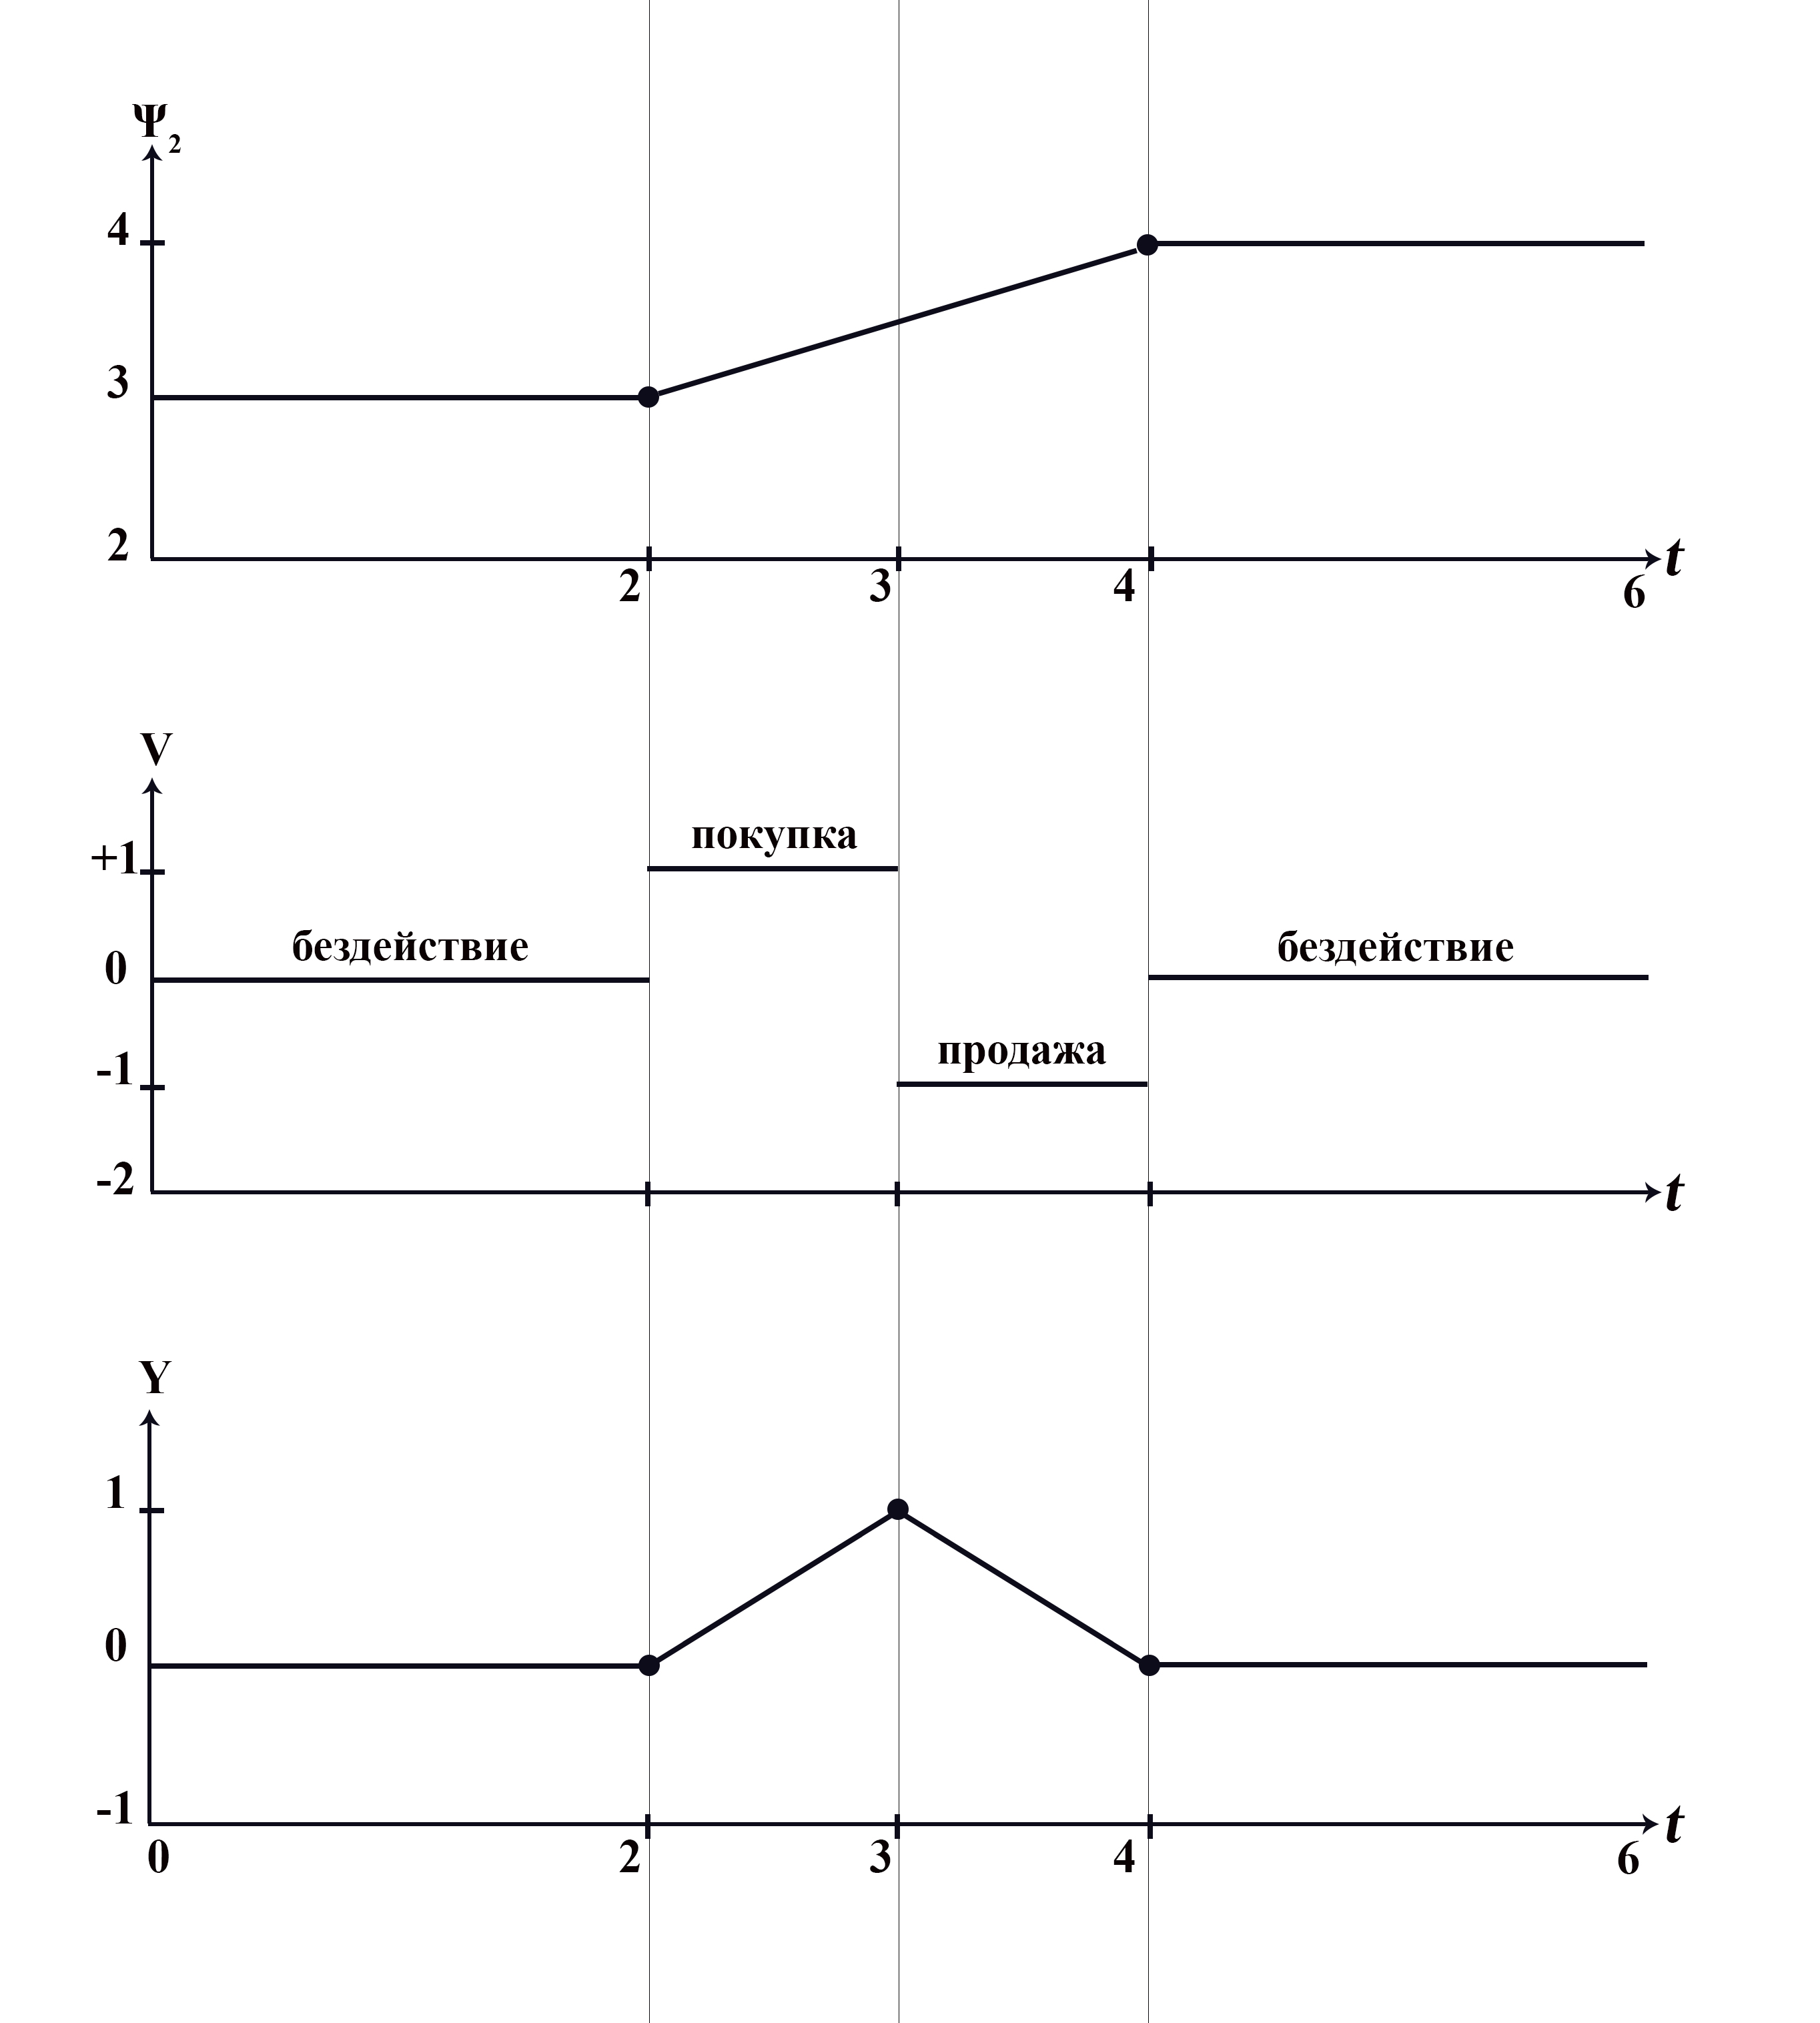
\includegraphics[scale=0.60]{images/gra.jpg}}
\caption{Стадии трейдинга в модели оптимального управления}
\end{figure}\label{ris:image}
\newpage

Заметим, что управление (\ref{f31}) и соответствующая траектория (\ref{f32}), (\ref{f33}) найдены в [8], с привлечением экономических соображений. Следуя упражнению 6.11 из [8] формально проверим управление $\overline{v}$ на экстремальность.


Управлению $\overline{v}$ соответствует сопряженная траектория $\overline{\psi_1} \equiv 1$,

\begin{gather*}
 \overline\psi_2 (t)=\left\{ \begin{array}{ll}
 3, & \textrm{при $ t \in [0, 2]$,}\\
 \frac{t}{2}+2, & \textrm{при $ t \in  (2, 4]$,}\\
  4, & \textrm{при $ t \in  (4, 6]$.}
  \end{array} \right.
\end{gather*}

Выпишем условие максимума функции Понтрягина для $(\overline{x}, \overline{y}, \overline{v})$ с $(\overline{\psi_1}, \overline{\psi_2})$ на каждом подотрезке времени с постоянным управлением.

На $\Delta_1 = [0, 2]$: 
\begin{gather*}
    (3 - 3) v \to \mathrm{max}, \,
    |v| \le 1.
\end{gather*}

На $\Delta_2 = (2, 3]$: 
\begin{gather*}
    (\frac{t}{2} - 1) v \to \mathrm{max}, \,  |v| \le 1;\\
\frac{t}{2} - 1 > 0.
\end{gather*}

На $\Delta_3 = (3, 4]$: 
\begin{gather*}
    (\frac{t}{2} - 2) v \to \mathrm{max}, \, |v| \le 1;\\
    \frac{t}{2} - 2 < 0 \, \textrm{при t<4.}
\end{gather*}

На $\Delta_4 = (4, 6]$: 
\begin{gather*}
    (4- 4) v \to \mathrm{max}, \,
    |v| \le 1.
\end{gather*}

Очевидно, что управление $\overline{v}$  ( вместе с $(\overline{x}, \overline{y}, \overline{\psi})$) удовлетворяет условию максимума, и следовательно, является экстремалью Понтрягина.

Установлено, что оптимальная стратегия позволяет увеличить общую стоимость активов с 10 до 10,5 денежных единиц в конечный момент времени по сравнению со стратегией бездействия трейдера. Причина этого состоит в том, что прогнозируемый скачок цены зерна дает возможность получить дополнительную выгоду при заданном уровне затрат на хранение пшеницы.


\mysubsection{Вариант задачи с квадратичной функцией $h$}

Изменим в исходной задаче значение функции затрат на хранение пшеницы  c ${h(y)} = \frac{1}{2}|y|$ на $ {h(y)} = \frac{1}{2} y^2 $\\

Наша задача запишется так:

\begin{align}
\mathcal{J} & = x(T) + p(T) y(T) \to \mathrm{max},\\
    \Dot{y} & = v, & y(t_{0}) = 0, \\
    \Dot{x} & = - \frac{1}{2} y^2 - p(t) v, & x(t_{0}) = 10.
\end{align}

Функция Понтрягина, сопряженная система и условия трансверсальности имеют вид: 
\begin{align}
    {H} & = \psi_{1} \big( - \frac{1}{2} y^2 - p(t) v \big) + \psi_{2} \big( v \big)\\
    \Dot{\psi_{1}} & = -H_x = 0 \Rightarrow \psi_1(t) \equiv 1, \\ \nonumber
    \Dot{\psi_{2}} & = -H_y = y \psi_{1} =y \Rightarrow \psi_{2}(6) = 4.\nonumber
\end{align} 


<<Bang-bang>>  определяется функцией переключения \\
$g = g(\psi_1 , \psi_2, p) = \big (\psi_{2} - p(t)\psi_{1} \big)$ и выглядит следующим образом:

\begin{align}
v^*(t) = 
 \begin{cases}
   1, &\text{ $\psi_{2} > p(t)$}\\
   -1, &\text{$\psi_{2} < p(t)$}\\
   \in [-1, 1], &\text{$\psi_{2} = p(t)$}
 \end{cases}
\end{align}

Основываясь на предыдущей задаче, выведем гипотезу, что оптимальное управление имеет структуру параметризации в моменты переключения. 
Зададим структуру управления с помощью параметров $\tau_1, \tau_2$:

\begin{align}
\overline v(t)=\left\{ \begin{array}{ll}
 0, & \textrm{при $ t \in [0, \tau_1],$}\\
 1, & \textrm{при $ t \in  [\tau_1, 3],$}\\
-1, & \textrm{при $ t \in  (3, \tau_2],$}\\
 0, & \textrm{при $ t \in  (\tau_2, 6];$}
  \end{array} \right.
\end{align}
Вычислим траектории:
\begin{align}
 \overline y(t)=\left\{ \begin{array}{ll}
 0, & \textrm{при $ t \in [0, \tau_1],$}\\
 t - \tau_1,  & \textrm{при $ t \in  [\tau_1, 3],$}\\
  -t + 6 - \tau_1, & \textrm{при $ t \in  (3, \tau_2],$}\\
   6 - \tau_2 - \tau_1,  & \textrm{при $ t \in (\tau_2, 6];$}
  \end{array} \right.
\end{align}

\begin{align}
 \Dot{x}(t)=\left\{ \begin{array}{ll}
 0, & \textrm{при $ t \in [0, \tau_1],$}\\
 -\frac{\big(t- \tau_1 \big)^2}{2} - 3, & \textrm{при $ t \in  [\tau_1, 3],$}\\
 -\frac{\big(6 - \tau_1 - t \big)^2}{2} + 4, & \textrm{при $ t \in  (3, \tau_2],$}\\
  -\frac{\big(6- \tau_1 - \tau_2 \big)^2}{2}, & \textrm{при $ t \in  (\tau_2, 6];$}
  \end{array} \right.
\end{align}



\begin{align}
 \overline x(t)=\left\{ \begin{array}{ll}
 10 ,& \textrm{при $ t \in [0, \tau_1],$}\\
-\frac{\big(t- \tau_1 \big)^3}{6} - 3t + 3 \tau_1 +10, & \textrm{при $ t \in   [\tau_1, 3],$}\\
  \frac{\big(6 -t- \tau_1 \big)^3}{6} + 4t - \frac{\big(3 - \tau_1 \big)^3}{3} - 11 + 3 \tau_1, & \textrm{при $ t \in   (3, \tau_2],$}\\
  - \frac{\big (6 - \tau_1 - \tau_2 \big )^ 2}{2}t + c, & \textrm{при $ t \in  (\tau_2, 6].$}
  \end{array} \right.
\end{align}

\begin{gather*}
 \overline x (3) = -\frac{\big(3- \tau_1 \big)^3}{3} - 9 + 3 \tau_1 + 10 = -\frac{\big(3- \tau_1 \big)^3}{6} + 12 + c,\\
 c =  -\frac{\big(3- \tau_1 \big)^3}{3} - 11 + 3 \tau_1 \\
   \overline x (\tau_2) = -\frac{\big(6- \tau_1 - \tau_2 \big)^3}{6} + 4 \tau_2 -\frac{\big(3- \tau_1 \big)^3}{3} - 11 + 3 \tau_1 =  -\frac{\big(6- \tau_1 - \tau_2 \big)^2}{2} \tau_1 + C,\\
   C = -\frac{\big(6- \tau_1 - \tau_2 \big)^3}{6} + \frac{\big(6- \tau_1 - \tau_2 \big)^2}{2} \tau_1 + 4 \tau_2 -\frac{\big(3- \tau_1 \big)^3}{3} - 11 + 3 \tau_1.
\end{gather*}


\begin{gather*}
\mathcal{J} = \Big[ 6 - \tau_2 - \tau_1 \Big]4 + \Big[ - 3 (6- \tau_1 - \tau_2)^2 + C \Big] \to \mathrm{max},\\
0 \leq \tau_1 \leq \tau_2 \leq 6.
\end{gather*}

Данная задача математического моделирования была решена с помощью системы  WolframAlpha \cite{s1}, \cite{s2} Рис.2. 

   
\begin{figure}[h]
\centering
%Рамка только для изображений с белым фоном
\fbox{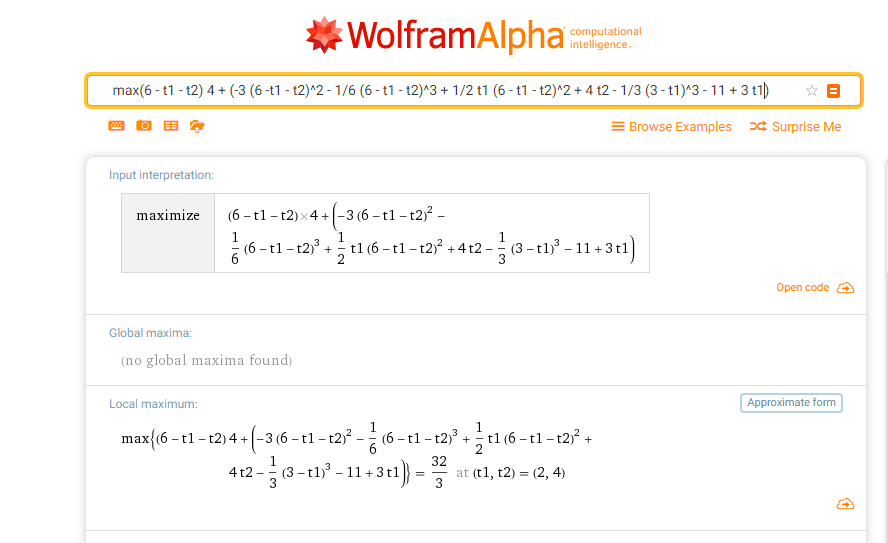
\includegraphics[scale=0.75]{images/d1.PNG}}
\caption{Решение с помощью системы WolframAlpha }
\end{figure}\label{p1}

%Очевидно, что  допустимо множество [0, 6], по теореме Вейерштрасса.


В следствие решения были получены значения $\tau_1 = 2, \tau_2 = 4$. Тогда управление и траектории запишутся следующим образом:

\begin{align}
\overline v(t)=\left\{ \begin{array}{ll}
 0, & \textrm{при $ t \in [0, 2],$}\\
 1, & \textrm{при $ t \in  [2, 3],$}\\
-1, & \textrm{при $ t \in  (3, 4],$}\\
 0, & \textrm{при $ t \in  (4, 6];$}
  \end{array} \right.
\end{align}

\begin{align}
 \overline y(t)=\left\{ \begin{array}{ll}
 0, & \textrm{при $ t \in [0, 2],$}\\
 t - 2,  & \textrm{при $ t \in  [2, 3],$}\\
  -t + 4, & \textrm{при $ t \in  (3, 4],$}\\
   0,  & \textrm{при $ t \in (4, 6];$}
  \end{array} \right.
\end{align}

\begin{align}
 \Dot{x}(t)=\left\{ \begin{array}{ll}
 0, & \textrm{при $ t \in [0, 2],$}\\
 -\frac{\big(t- 2 \big)^2}{2} - 3, & \textrm{при $ t \in  [2, 3],$}\\
 -\frac{\big(4 - t \big)^2}{2} + 4, & \textrm{при $ t \in  (3, 4],$}\\
  0, & \textrm{при $ t \in  (4, 6];$}
  \end{array} \right.
\end{align}

\begin{align}
 \overline x(t)=\left\{ \begin{array}{ll}
 10, & \textrm{при $ t \in [0, 2],$}\\
6 \frac{5}{6}, & \textrm{при $ t \in [2, 3],$}\\
10 \frac{1}{3},  & \textrm{при $ t \in   (3, 4],$}\\
 10 \frac{2}{3}, & \textrm{при $ t \in  (4, 6].$}
  \end{array} \right.
\end{align}


Получим, что $\overline{J} =  10 \frac{2}{3}$. Проверим этот процесс на экстремальность с помощью Принципа максимума.


Управлению $\overline{v}$ соответствует сопряженная траектория $\overline{\psi_1} \equiv 1$,

\begin{gather*}
 \overline\psi_2 (t)=\left\{ \begin{array}{ll}
 3, & \textrm{при $ t \in [0, 2]$,}\\
 \frac{t^2}{2}- 2t+5, & \textrm{при $ t \in  (2, 3]$,}\\
 -\frac{t^2}{2}+4t-4, & \textrm{при $ t \in  (3, 4]$,}\\
  4, & \textrm{при $ t \in  (4, 6]$.}
  \end{array} \right.
\end{gather*}

График функций  $( \overline{y}, \overline{v}, \overline{\psi_2})$ на каждом интервале времени с постоянным управлением. Рис.3.


\begin{figure}[h]
\centering
%Рамка только для изображений с белым фоном
\fbox{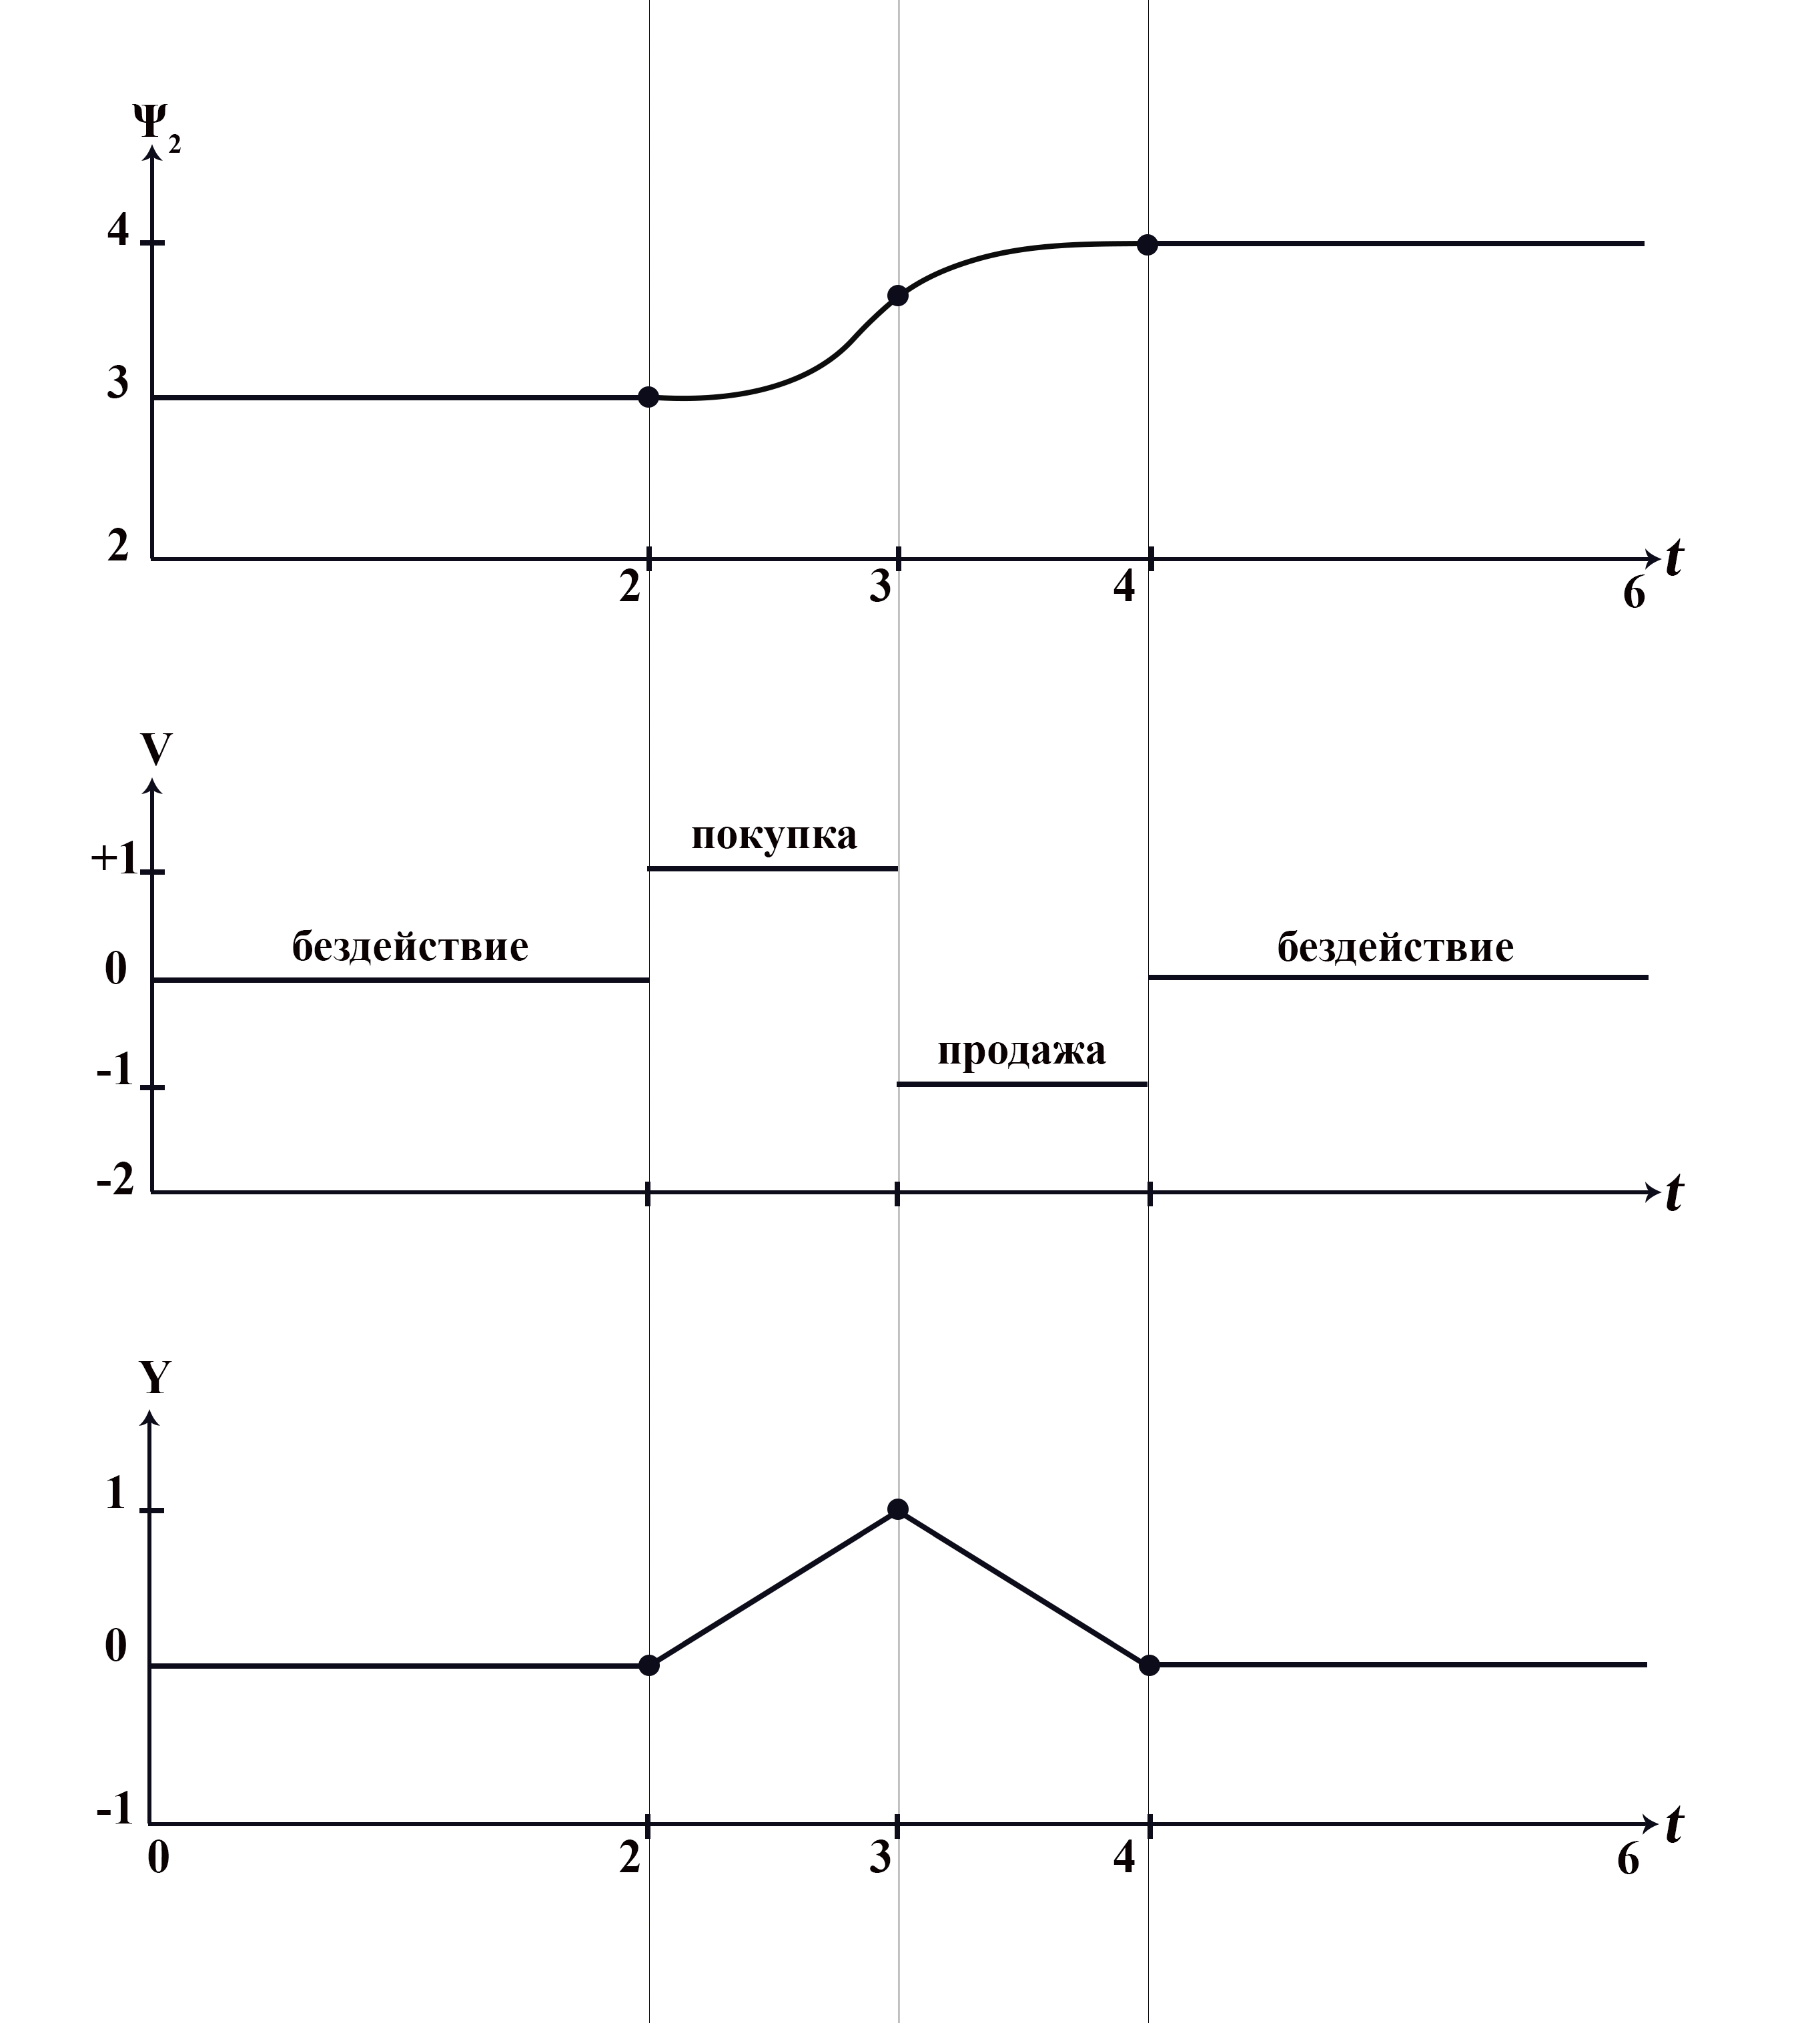
\includegraphics[scale=0.60]{images/grafiki.jpg}}
\caption{Стадии трейдинга в модели оптимального управления }
\end{figure}

Выпишем условие максимума функции Понтрягина для $(\overline{x}, \overline{y}, \overline{v})$ с $(\overline{\psi_1}, \overline{\psi_2})$ на каждом подотрезке времени с постоянным управлением.


На $\Delta_1 = [0, 2]$: 
\begin{gather*}
    (3 - 3) v \to \mathrm{max}, \,
    |v| \le 1.
\end{gather*}

На $\Delta_2 = (2, 3]$: 
\begin{gather*}
    (\frac{t^2}{2} - 2t + 2) v \to \mathrm{max}, \,  |v| \le 1;\\
\frac{t^2}{2} - 2t +2 > 0.
\end{gather*}

На $\Delta_3 = (3, 4]$: 
\begin{gather*}
    (-\frac{t^2}{2} + 4t - 8) v \to \mathrm{max}, \, |v| \le 1;\\
   - \frac{t^2}{2}+4t - 8 < 0, \, \textrm{ при $t<4$}.
\end{gather*}

На $\Delta_4 = (4, 6]$: 
\begin{gather*}
    (4- 4) v \to \mathrm{max}, \,
    |v| \le 1.
\end{gather*}

Очевидно, что управление $\overline{v}$  ( вместе с $(\overline{x}, \overline{y}, \overline{\psi})$) подозрительно на оптимальность, и следовательно, является экстремалью Понтрягина.

Установлено, что оптимальная стратегия позволяет увеличить общую стоимость активов с 10 до $10\frac{2}{3}$ денежных единиц в конечный момент времени по сравнению со стратегией бездействия трейдера. Причина этого состоит в том, что прогнозируемый скачок цены зерна дает возможность получить дополнительную выгоду при заданном уровне затрат на хранение пшеницы.
